\section{Implémentation}
\label{sec:implementation}
  
  % Utilisation d'un analyseur sémantique de fichiers exécutables pour la
  % reconstruction de CFG.

  Notre outil manipule des fichiers binaires exécutables compilés pour des
  cibles embarquées à base de microprocesseurs PowerPC. Les informations
  nécessaires à la reconstruction d'un CFG et au \emph{program slicing} sont
  issues d'un outil généré par HARMLESS \cite{KBB12}, un générateur
  de simulateurs basé sur un HDL.

  \begin{figure}[ht]
    \centering
    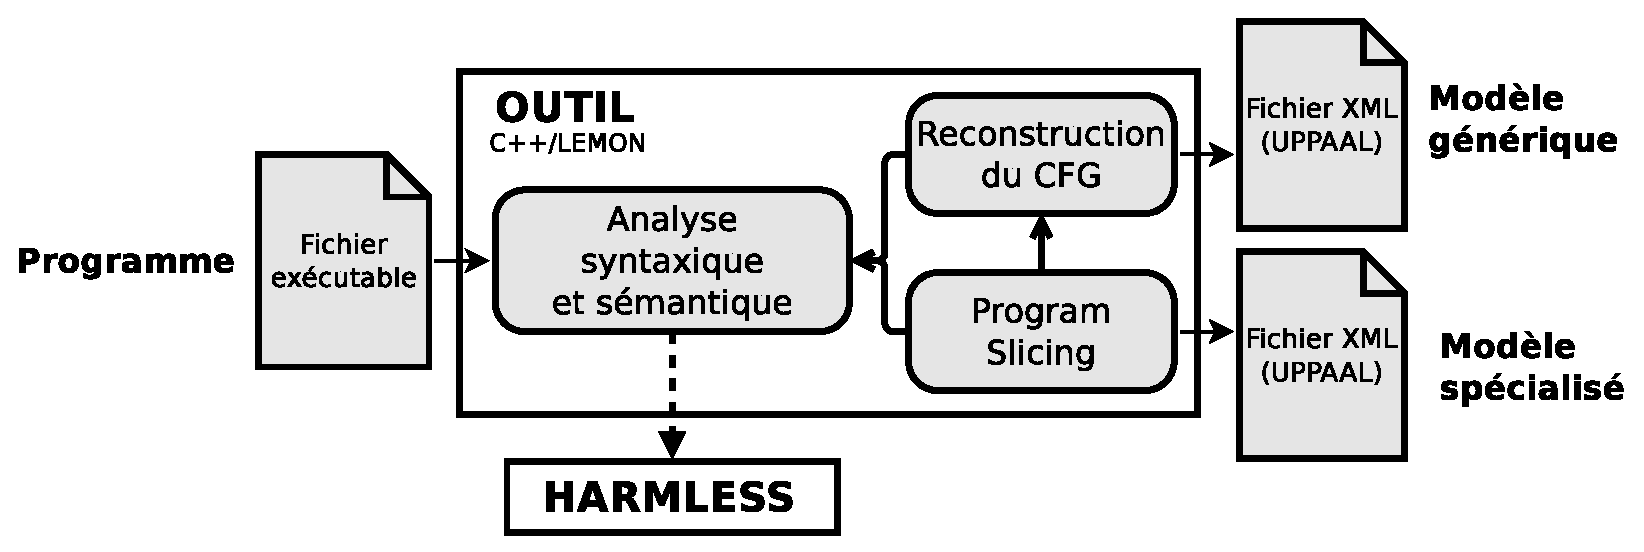
\includegraphics[scale=.3]{img/archi.eps}
    \caption{Structuration de l'outil}
    \label{fig:implem}
  \end{figure}

  %% Utilisation de la propagation de constante pour rafiner le CFG.
    
  %% Afin de permettre la déterminaison de certaines cibles de saut il est une
  %% nouvelle fois fait usage de l'outil HARMLESS. Celui-ci réalise une
  %% simulation de l'exécution de notre programme sur la plateforme matérielle
  %% considérée. Il est donc possible de procéder à une propagation de constantes
  %% permettant de déterminer des plages de valeurs pour certains registres.

  Notre outil est développé en C++. Il s'appuie sur la bibliothèque de
  manipulation de graphe LEMON~\cite{DJK11}. Les modèles du programme obtenus avant
  ou après \emph{slicing} peuvent être exporter au format Dot, pour être
  visualisés, ainsi que sous forme d'automates temporisés au format
  UPPAAL~\cite{LPY97}.
  %Pour valider l'outil, nous avons réalisé différents tests à partir des \emph{benchmarks} de Mälardalen
  %\cite{malardalen-bench}.

  %Ces \emph{benchmarks} sont utilisés pour évaluer et comparer
  %différents outils et méthodes de calcul de pire cas de temps d'exécution.
